% Q21：按固定候选 PDF 第 2 页重绘椭圆、弦 AB、中点 P、过 F 的直线 m 与右准线 l；比例为示意。
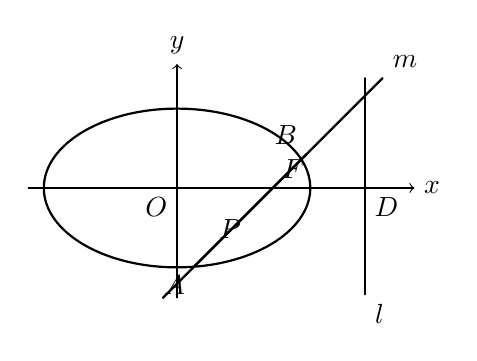
\begin{tikzpicture}[line cap=round,line join=round,scale=0.9]
  \coordinate (O) at (0,0);
  \coordinate (F) at (1.35,0);
  \coordinate (D) at (2.65,0);
  \coordinate (A) at (0.25,-1.10);
  \coordinate (B) at (1.83,0.48);
  \coordinate (P) at (1.04,-0.31);

  \draw[->] (-2.1,0)--(3.35,0) node[right] {$x$};
  \draw[->] (0,-1.55)--(0,1.75) node[above] {$y$};
  \draw[thick] (O) ellipse (1.88 and 1.12);
  \draw[thick] (-0.2,-1.55)--(2.9,1.55) node[above right] {$m$};
  \draw[thick] (A)--(B);
  \draw[thick] (2.65,-1.5)--(2.65,1.55) node[below right] at (2.65,-1.5) {$l$};

  \node[below left] at (O) {$O$};
  \node[above right] at (F) {$F$};
  \node[above left] at (B) {$B$};
  \node[below left] at (A) {$A$};
  \node[below left] at (P) {$P$};
  \node[below right] at (D) {$D$};
\end{tikzpicture}
